%\section{Related Work}\label{Related}

	近年來許多不同的技術運用在室內定位上,像是無線網路、藍芽及RFID等相關技術領域,但都受到環境的阻隔與訊號間的干擾,使得無法做到精準的定位。之後在提出
相關影像定位的研究,利用影像特徵替代訊號,解決了訊號干擾的問題,但不足的地方在於特定拍照的區域上才能做到有效的定位。在我們的方法裡,提出利用重建3D定位環境,將3D
環境投影成平面虛擬影像,利用虛擬影像比對特徵定位。根據參考\cite{Muthukrishnan05}的室內定位方式分析,根據表 \ref{table:Indoor Localization analysis Table}
比較各個室內定位方式所花費的成本做分析,可以得知,影像定位可以花較少的成本得到最高的精確度。
在下面相關研究的章節裡,首先在2.1介紹先關影像定位的研究,在2.2節裡介紹3D環境重建的方法,2.3介紹
將3D影像投影成平面影像相關技術的應用,最後說明如何將這些研究帶到我們的方法裡。

\begin{table}[htbp]
  \centering
  \caption{室內定位實驗所需設備成本與精確度比較}
    \begin{tabular}{rrrr}
    \toprule
    定位技術 :  & 定位精確度 & 所需花費  &  實驗難易度 \\
    \midrule
    紅外線 :  &  5-10 m & 高 & 中等 \\
    RFID  :  &  1-10 m & 高 & 中等 \\
    Wi-Fi :  &  5 cm-5 m & 高 & 高 \\
    手持攝影機 :  & 1- 5 m  & 低 & 中等 \\
    監控攝影機 :  & 10 cm-1 m & 高 & 低  analysis \\
    \bottomrule
    \end{tabular}%
  \label{table:Indoor Localization analysis Table}%
\end{table}%


\section{平面影像定位類型分析}
%介紹影像定位不同的區分
	定位研究有許多應用在影像視覺與機器人的領域上,不同的地方在於他們如何擷取特徵作應用。像是Junqiu Wang在2004年利用Harris-Lapalace	
角點偵測,將相片存取資料庫中,根據特徵點多寡投票找出最相似的照片,再將相機紀錄照片的座標位置作矩陣分解,推測出待定位照片的位置。Andreasson
在2005年\cite{Andreasson2005}利用全景鏡頭大範圍且廣角的特性,把SIFT擷取的特徵點作為Particle Filter的輸入條件,追蹤照片位置
做定位。Timothy Liu在2010年\cite{LiuT2010}將雷射與攝影機作結合,蒐集深度資料作為之後定位參考的依據。藉由定位方法依據的不同,或是
使用輔助感測器提升定位的效果,使得影像定位在許多領域上有不同的運用。

%定位的方式不同
	更深入來看影像定位,有不同的定位方式,根據Bonin-Font等人的\cite{Bonin-Font2008}的歷年來的研究分析,主要把定位方式分成三大類,三角定位(Triangulation),
馬可夫鏈(Markov)與粒子濾波器(Particle Filter)。
三角定位傳統運用於GPS上,依據發射器訊號的角度與位置,透過餘弦定理找出這些位置的關係式,將這些關係式帶入最小平方法(Least Square)求解。應用在影像定位來看,
把影像特徵點取代為GPS的訊號,根據特徵點與相機的角度及特徵點的位置當作三角定位的輸入條件。像是Dana Cobzas\cite{Cobzas2003},利用雷射讀取影像的深度,
比對2D影像的特徵點,根據特徵點與相機的夾角與位置等資訊求取初步的定位資訊,再根據影像深度的關係更新定位點所在的資訊,得到最後的定位成果。在這篇方法將三角定位與影像
特徵比對作應用整合,但礙於特徵點比對的方法不夠精細,使得定位精確度受到影響,在我們的方法上使用SIFT更精確的特徵點比對方式,使得定位結果獲得改善。

	也有的研究將馬可夫鏈(Markov)的特性運用在影像定位上,像是Morita等人\cite{Morita2005}利用兩層SVM(Support Vector Machine)判斷出影像所在的位置區域,再利用馬可
夫鏈根據歷史紀錄作推測出Support Vector Machine(SVM)所求的位置是否準確。馬可夫鏈是一套機率統計模型,藉由之前機率分布的狀況,推測出未來可能發生的機率分布。在這
裡是增進SVM的定位效果,也可以減少SVM的訓練成本。大部分馬可夫鏈的研究室運用於導航上,因為需要大量的樣本數來推估機率模型,機器人導航藉由紀錄路徑中的大量影像來推測機
率模型相當適合,但是少許的照片樣本數對定位效果的幫助並不顯著,所以對於室內定位小範圍且高密度的定位系統來看,Markov較不適用於小範圍的定位應用。

	粒子濾波器(Particle Filter)或稱為Monte Carlo定位方法,將拍攝影像存為樣本數,依據影像重複出現的特徵次數給予權重,根據不同的權重值分類,當下一次新的影像
輸入時,比對相同的影像特徵所出現的次數,分類到所屬的權重值。在不同的Monte Carlo定位研究中,因為所取出特徵點的特性不同,而有不同方式的定位應用。像是在Jürgen Wolf
等人的研究中\cite{Wolf2005},利用紅、綠、藍三原色的像素統計直方圖當作特徵點,依據不同的權重做分類找出定位的所在地。Monte Carlo可以做大範圍的地圖定位,但是
事先需要地圖的輔助,所以不適用我們的方法。

	根據三種不同的定位方式,我們找出三角定位最適合於我們的方法上,因為不需要大量的影像資料作輔助,也不用事先地圖作記錄。藉由點雲環境投影至平面的虛擬影像,當作資料庫的
資料來源,這些影像位置不需事先的測量,節省人工紀錄的時間成本,也不用將影像事先作分類,減少訓練的成本。
	
\section{3D環境重建技術}

	3D環境重建在視覺定位上的研究。在這小節裡,先說明利用RGB-D 感測器建置3D環境的研究,接下來參考相關
Visual SLAM的研究,以及說明我們所實作調整與最佳化點雲環境的演算法-Sparse Pose Adjustment。
	
\subsection{RGB-D Mapping 3D環境建置}
			
\begin{figure*}
\begin{center}
  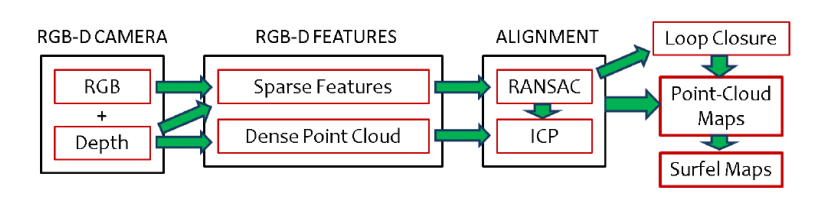
\includegraphics[width=1.0\textwidth]{figures/RGB-D_System_Overview.eps}
  \caption{\cite{Henry2012}RGB-D環境建置流程示意圖}
  \label{fig:RGB-D System}
\end{center}
\end{figure*} 
							
	 在Peter Henry等人\cite{Henry2012}的研究中,利用可偵測深度的攝影機來建置3D點雲環境。以圖\ref{fig:RGB-D System}說明整個點雲建置流程分為三大步驟,第一階段首先擷取攝影機畫面,第二階段取出畫面中的特徵與
深度作比對,最後階段根據特徵點群先作RANSAC(隨機一致演算法)求取最好的轉換矩陣後,再根據ICP把點雲之間作最小化誤差。在我們的研究中,參考了\cite{Henry2012}建置環境的作法,但為了減
少運算時間,在我們的方法裡把每個影格作Iterative Closet Point(ICP)的時間,移置到最後階段作最佳化。在下面的小節裡,我們將介紹這篇研究中如何將RGB-D攝影機擷取的特徵作比對,以及最小化點雲
距離誤差的方法。

\begin{algorithm}[htb] 
\renewcommand{\algorithmicrequire}{\textbf{Input:}}
\renewcommand\algorithmicensure {\textbf{Output:} }
\caption{ RGBD-ICP: } %算法的標題
	\label{alg:RGBD-ICP} %给算法一個標籤,这样方便在文中對演算法的引用
	\begin{algorithmic}[1] %這個1 表示每一行都顯示数字
	\REQUIRE ~~\\ %演算法的输入参数:Input
	RGB-D Frame, $P_s$;\\
	The Target Frame, $P_t$;\\
	\ENSURE ~~\\ %演算法的输出:Output
	Transformation Matrix, $t^*$;\\

	\STATE $F$=Extract$\_$RGBPoint$\_$Feature($P_s$) \label{code:extract_feature_f1} 
	\STATE $F_{target}$=Extract$\_$RGBPoint$\_$Feature($P_t$) \label{code:extract_feature_f2}
	\STATE ($t^*$, $A_f$)=Perform$\_$RANSAC$\_$Alignment($F$,$F_{target}$) \label{code:RANSAC}
	\REPEAT \label{code:into while}
		\STATE $A_d$ = Compute$\_$Closet$\_$Points($t^*$,$P_s$,$P_t$) \label{code:Compute ICP}
		\STATE $t^*$ = $argmin_t \alpha$($\frac{1}{|A_f|}\sum_{i \epsilon A_f} w_i|t(f_s^i)-f_t^j|^2$) + ($1-\alpha$)($\frac{1}{|A_d|}\sum_{j \epsilon A_d} w_j|(t(P_s^i)-P_t^j)\cdot n_t^j|^2$) \label{code:Compute Minimal Distance Error}
	\UNTIL{($Error \_ Change(t^*) \leq \theta$) or ($maxIter \_ reached$)} \label{code:Exit While}
	\RETURN $t^*$; %演算法的返回值
\end{algorithmic}
\end{algorithm}

	演算法\ref{alg:RGBD-ICP}說明如何將RGB-D攝影機擷取到的影格畫面,做點雲的重合與矯正。在上述的演算法中,透過前一秒的影格與下一秒的影格畫面當作輸入來源,先利用RANSAC作
找出初始化的轉移矩陣,再進入迴圈利用ICP作轉移矩陣的最佳化,當誤差值小於等於$\theta$值或達到最大迭代次數時,結束演算法。Step \ref{code:extract_feature_f1} 與Step \ref{code:extract_feature_f2} 利用SIFT作特徵點比對,在擷取影格中對應的特徵點與深度值。當擷取完特徵點與深度值中,帶入Step \ref{code:RANSAC} 中,求取初始的轉移矩陣,
透過RANSAC的演算法,找出剩下特徵點群中屬於inlier的數量,把這個數量當作迭代次數當作其中一個ICP的中止條件。RANSAC除了找出初始的轉移矩陣及inliers的數目之外,還可以找出存在這個
轉移矩陣中最好的特徵點配對關係。根據這個配對關係,帶入接下來的ICP流程中求取點雲距離誤差最小化。
	
	Step \ref{code:into while}-Step \ref{code:Exit While}進入到ICP的流程裡面,並根據權重找出最佳的轉移矩陣解。首先在Steps \ref{code:Compute ICP} 中根據
$t^*$轉換矩陣的的轉換後,計算點雲跟點雲之間的配對關係,並找出在點雲$P_s$中跟點雲$P_t$距離最近的點群。當找出距離最近的點群之後,根據Steps \ref{code:Compute Minimal Distance
Error} 的式子,計算點群間最小距離的誤差,判斷是否小於等於$\theta$值當作離開ICP的條件。這項式子分成兩部分所組成,第一部分計算RANSAC轉移後點雲之間的距離,第二部分計算ICP算出來點
群之間的誤差值,利用權重分配最適合的轉移矩陣解。為的使算出來誤差衡量具有公平性,在第二部分裡算點雲誤差乘上normal值${n_t^j}$,使得與第一部分維持一樣的比例,${n_t^j}$是在點雲$P_t$
根據主成分分析(Principle Component Analysis)所算出來的集合值。當達到Steps \ref{code:Exit While} 的完成條件,最後回傳$t^*$轉換矩陣,利用轉換矩陣將點帶入矩陣中,進行點雲間
的重和與調整。

	\cite{Henry2012}的方法提供了RGBD-ICP演算法,這套演算法幫助了RANSAC達到了更精確的重合效果,但是也增加了運算的時間,在我們的方法裡參考了前半部RANSAC轉移矩陣的求解過程,
之後對於點雲誤差距離最小化的問題,參考了解決Visual SLAM問題在誤差距離最小化過程的解法。下面小節先探討Visual SLAM問題描述,以及解決Visual SLAM問題在建置3D環境下有哪些幫助。
	
\subsection{Visual SLAM的問題描述與在建置3D環境的應用}

%描述VSLAM的相關問題
	Simultaneous Localization And Mapping(SLAM)描述的是記錄拍攝路徑的連續影像,利用影像的相對關係來製作環境地圖,適合用來做探勘環境,機器人導航、定位
等用途。Visual SLAM將SLAM技術與電腦視覺作結合,透過雷射、kinect或具備深度感測的儀器,達到建置環境地圖的目的,更能夠透過電腦視覺重現原來環境的樣貌。我們利用解決
Visual SLAM問題的作法,透過拍攝室內環境的照片,利用照片重建定位環境。在下面的小節裡,描述現在那些技術能夠解決Visual SLAM的問題,及這些技術怎麼幫助在建置3D環境上。

	在Jorge Fuentes-Pacheo等人的相關研究\cite{Fuentes-Pacheco2012}中,根據Visual SLAM會遇到的問題,提出了三個分類:地圖封閉檢測(Loop closure detection)、
無法辨識所在位置(Kidnapped robot)與多重地圖重合(Multi-session and cooperative mapping)。地圖封閉檢測描述的問題是,當機器人導航或者是利用攝影機建置地圖時,回到起始點時
能否檢測出封閉性。舉一個例子來講,像是建房間地圖時,從大門開始環繞四周牆壁,當回到大門時,能否判斷大門的位置為一開始的起始點,完成地圖的封閉性。在Kin Leong Ho等人的研究中
\cite{Ho2007}根據影像辨識的方法,先將影像的特徵比對結果成對記錄成對稱矩陣,再利用SVD(Single Value Deco3mposition)分解進行主成分分析(PCA),辨識是否為相識的影像,如果是
則完成建置地圖。Eade等人在2007年的研究中\cite{Eade2007},將他們解決momocular Visual SLAM的方法稱為Graph SLAM,作法是將每個攝影機的位置作紀錄,在這些紀錄點儲存景物
特徵點的資訊,將之前紀錄點建置機率模型,當下一個紀錄點在紀錄時,預測這個紀錄點是否出現在之前紀錄所在的位置,或是這個紀錄點跟之前的紀錄點是否相關,來偵測封閉性或是減少建置地圖失
敗的情形發生。

	無法辨識所在位置,問題發生在機器缺乏之前環境位置的資訊,無法辨識目前位置,或是機器突然被轉移到別處,雖然已經有環境資訊,卻還是無法辨識現在的下落,也有的情形像是機器遇到障礙物,
因為無法辨識障礙物,導致機器發生錯誤判斷的情形發生。在Denis Chekhlov等人的研究中\cite{Chekhlov2008},提出一個可以容錯且還原SLAM錯誤的系統機制。他們在紀錄點建立目次順序,並且在
不同的解析度找出SIFT特徵點供辨識參考,在缺乏現有環境資訊的狀態下,能從之前的的紀錄點推測出現在的位置,達到容錯的效果。

	多重地圖重合,當在不只使用一個機器人或是攝影機的情況下,需要將多張地圖對齊拼貼成一張完整的地圖,在許多相關的研究,如Ho和Newman等人的研究\cite{Ho2007}、及Gil等人的的研究
\cite{Gil2010},都曾在研究中探討過相關的問題,這些解法大部分都是找出最近的鄰居(Nearest Neighbour)或者是聯合相容分枝定界(Joint Compatibility Branch and Bound)的解法。
這些解法相似的地方在於一開始必須對機器人的位置做很相近的猜測,如果與起始點差異過大,就會發生地圖碎裂或者是重疊的情況產生。

%相關VSLAM 的研究
	在我們的研究中,根據地圖封閉檢測這個問題作延伸,探討如何在建立點雲環境中能夠封閉重和。有關這類問題,在減少3D投影誤差及作出重合最佳化的研究,稱為Bundle 
Adjustment(BA)\cite{Triggs2000},我們針對這類的演算法,找出相關論文中最適用於我們的研究的演算法-Sparse Pose Adjustment演算法。

\begin{figure*}
\begin{center}
  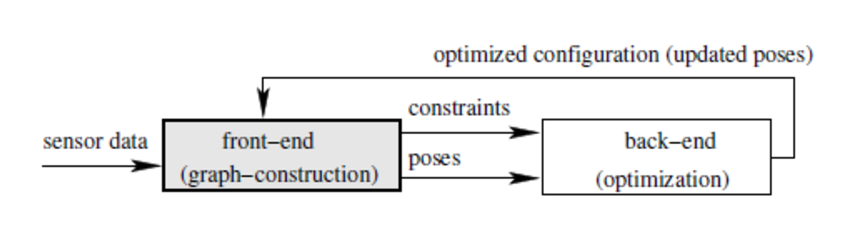
\includegraphics[width=1.0\textwidth]{figures/Graph-based_SLAM.eps}
  \caption{\cite{Konolige2010}Graph-based SLAM系統,透過新的pose帶入不斷更新}
  \label{fig:RGB-D System}
\end{center}

\end{figure*}  

%介紹在本篇所用的Sparse Pose Adjustment
	為了將3D模型做出效果能更逼近真實並且能達到封閉,Kurt Konnolige等人將BA的概念運用在SLAM上\cite{Konolige2010}。以圖\ref{fig:RGB-D System}為例,將輸入的資料透過攝影機的條件予以限制,
利用這些限制條件來達到Graph SLAM完成最佳化的條件做出了更有效率的最佳化,稱為Sparse Pose Adjustment(SPA),藉由輸入攝影機或是感測器位置以及角度的資訊,作成協方差矩陣(Covariance Matrix)
,利用協方差矩陣為Levenberg-Marquardt的限制條件(Constraint),再利用迭代法將誤差降到最小,達到最佳化的條件。

\section{3D投影平面深度內插研究}
                                                                                                                                                                                                                                                                                                                                                                                                                                                                                                                                                                                                                                                                                                                                                                                                                                                                                                                                                                                                                                                                                                                                                                                                                                                                                                                                                                                                                                                                                                                                                                                                                                                                                                                                                                                                                                                                                                                                                                                                                                                                                                                                                                                                                                                                                                                                                                                                                                                                                                                                                                                                                                                                                                                                                                                                                                                                                                                                                                                                                                                                                                                                                                                                                                                                                                                                                                                                                                                                                                                                                                                                                                                                                                                                                                                                                                                                                                                                                                                                                                                                                                                                                                                                                                                               
	在3D投影的相關研究上,有的研究將3D投影作補強\cite{Zhang2010}\cite{Riecher2012},對影像作深度內插法以及高斯濾波器(Gaussian Filter)作平滑處理,防止投影出來的
平面碎裂化,在應用方面可以用來幫助3D模型作更好的影像渲染(image rendering)。在我們的方法中也參考了深度內插法補強的部分,防止因為深度錯誤而導致圖形碎裂的情形發生,增加虛擬
影像特徵辨識的能力。

	在Byong Mok Oh的研究中\cite{Oh2001},提供了一個很有趣的想法,利用畫素的深度來作視角轉換,透過這些深度作出轉移矩陣(homography),模擬這些畫面在視角上的變換,不過
因為當時深度偵測的儀器並不普及,只能夠利用陰影模擬深度變化,所以作出來的模擬畫面與真實畫面有些差距,但是利用深度作照片編輯與改變照片視角,是一個很有趣的應用,在本篇研究中把這
個想法運用到畫面深度的測量,當影像深度buffer過大時代表相機離物體距離過近,我們將相機視角隨機往左邊或右邊轉角度避過障礙物或環境邊緣,使得照片包含更多關於環境上的資訊。
	
	也有的研究把平面影像投影成3D深度畫面,像是Chenglei Wu在2012年\cite{Dichangsheng2012}追蹤影片中的物體的行動,在non-keyframe的時候取出追蹤物體取出深度,當在key 
frame時賦予追蹤物體深度,可以做出取出前景的效果,也可以把深度拿來製作3D景深。其中被物體擋住的深度利用內插法,將其他non-keyframe的深度補齊至keyframe中。把影像追中與深度偵
測結合再一起,成為一個新的方法提出,但一旦背景複雜,就無法利用內插法補齊差值,所以容錯能力成為此類研究的改進目標。	

	在接下來的章節參考上述的相關研究方法,在室內影像定位做技術的整合與改良。在我們的方法利用內插法補族缺陷的照片深度,並參考照片的深度決定虛擬相機拍攝的角度,最後利用影像資料庫
內的照片做定位比對。我們使用定位的方法為三角定位,取決於不需要額外的訓練成本,在藉由深度儀器的輔助下,找出比一般照片更充足的影像特徵,也彌補拍攝影像位置取樣的不足,最後與傳統影像
定位做比較,針對覆蓋率與精準度對室內環境做定位測試分析。	


%\section{特徵點的比對與匹配}
%
%	建置3D模型中,我們的方法利用Graph SLAM方法來減少相片之間匹配的錯誤,在上個章節介紹了SLAM的相關研究後,在這個章節我們將說明
%如何利用照片找出特徵點,及特徵點匹配的相關研究。找出圖形特徵點及匹配特徵點,目的在不同的照片中拍攝到相同的景物,利用同樣的景物找出兩
%個照片相對應的特徵點,再利用特徵點求出這些相片的的相對位置,決定如何將照片放置在3D環境中。基於這項目的,先利用SIFT找出特徵點,再用
%RANSAC找出特徵點匹配的關係,使得照片能夠在正確的位置重合。下面的章節將介紹SIFT與RANSAC的方法。
%	
%\subsection{SIFT 尺度不變特徵向量}
%SIFT 特徵點描述方法
%	取出相片中特徵點的方法,一開始由 lowe \cite{Lowe2004} 所提出,稱為尺度不變特徵向量(SIFT)。後來有人針對SIFT做演算法的加速
%(SURF)\cite{Bay2006}以及增強找出特徵點數量的方法(ASIFT)\cite{Guo2009}。SURF的方法雖然快速,但是簡化許多計算流程,影響找出
%圖片當中特徵點的數量,如果套用在我們的方法中,會導致之後特徵點無法做到有效的匹配。ASIFT是將照片可能會旋轉、放大或縮小的情況考慮進去
%,將這些照片模擬不同變化,再根據不同變化的照片中找出匹配的特徵點。此舉會導致運算量的增加,考慮到龐大的運算量導致時間的增加,我們還是
%使用一般的SIFT方法找出特徵點。
%
%	尺度不變特徵向量(SIFT),主要分成四個階段:
%
% \begin{enumerate}
%	  \item 區域空間極值分布	
%	  \item 特徵點定位與篩選
%	  \item 特徵點方向分配
%	  \item 特徵點描述向量建立
% \end{enumerate}
%
%   第一階段(1) 區域空間極值篩選,先利用不同尺度間的高斯金字塔選擇區域中的最大極值,其高斯分布式子如下:
%\begin{align}
%  G(x,y,\sigma) = \frac{1}{2\pi\sigma^2}exp(-(x^2+y^2)/2\sigma^2) 
%\end{align}
%
%	不同尺度的高斯分布利用摺積 (Convolution) 將影像模糊化。 $I(x,y)$代表原始影像,$G(x,y,\sigma)$代表高斯函數:	
%\begin{align}
%  L(x,y,\sigma) = G(x,y,\sigma)\ast{I(x,y)}
%\end{align}
%
%\begin{figure}
%  \begin{center}
%    \subfigure[高斯差分與影像金字塔]{\label{fig:Gaussian Prymaid}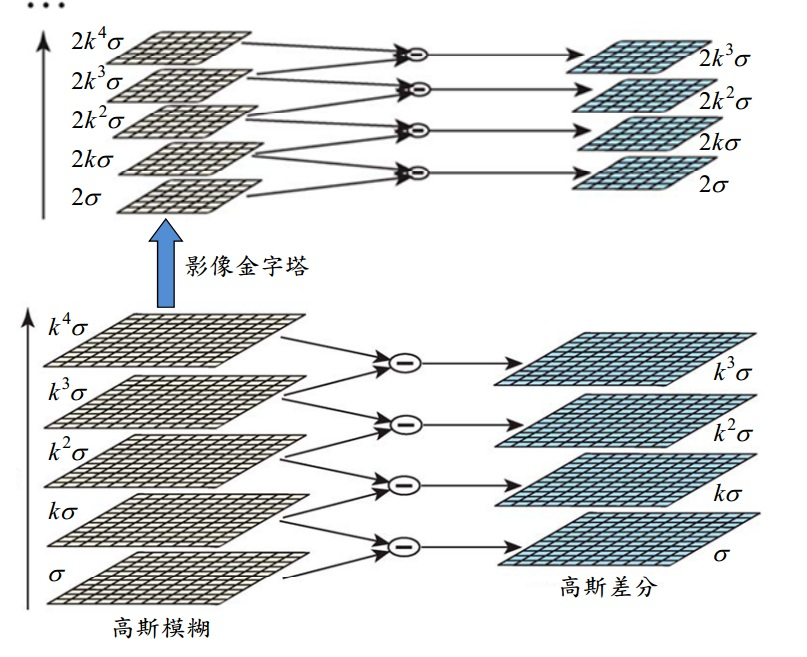
\includegraphics[width=0.45\columnwidth]{figures/Gaussian_Prymaid.jpg}}
%    \subfigure[尺度極值偵測]{\label{fig:Extreme Value Detect}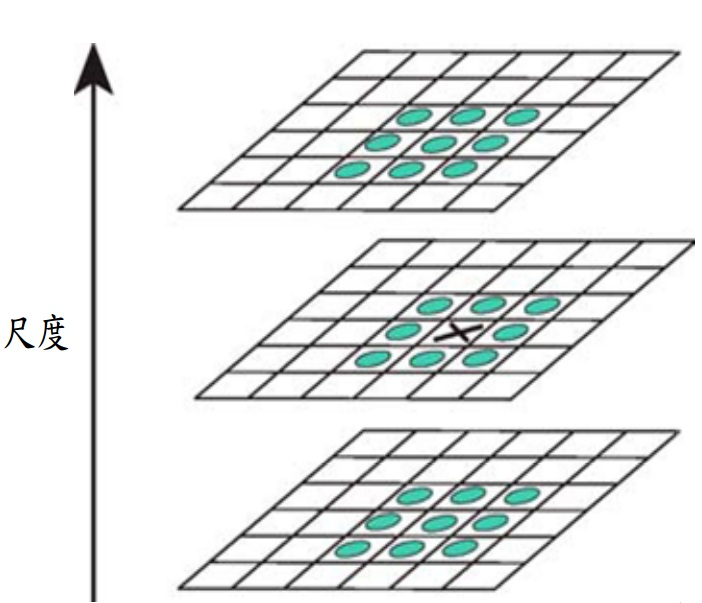
\includegraphics[width=0.45\columnwidth]{figures/extreme_value_detect.jpg}}
%  \end{center}
%  \caption{glFrustrum 矩陣圖示說明}
%  \label{fig:SIFT_explanation}
%\end{figure}
%
%  再利用每組影像相鄰的高絲模糊影像進行高斯差分(Difference-Of-Gaussian),目的用於在集合內4組高斯差分影像中找出極值
%  ,式子如(1.3)所示:    
%\begin{align}
%  D(x,y,\sigma) = L(x,y,k\sigma)-L(x,y,\sigma)
%\end{align}
%
%  在此k為高斯模糊的尺度比值,設為$\sqrt{2}$,若某個像素的極值為26個相鄰的像素中最大或最小的話,則此像素的位址即為區域極值的所在。
%
%  第二階段(2) 特徵點定位篩選,其主要的目的在於找出真正有用的特徵點,在此特徵點的精準度必須要達到次像素的精度。有的特徵點其極值為低對比度的點,這時候這些低對比度的特徵點
%就會不予採用,剩下的特徵點即可為下一階段所使用。作法首先將(1.3)利用泰勒展開得到(1.4): 
%\begin{align}
%  D(x) = D + \frac{\delta D^T}{\delta X}X + \frac{1}{2}X^T\frac{\delta^2 D}{\delta X^2}X
%\end{align}
%
%   式中$X$為極值$(x,y,\delta)^T$,$D$為高斯差分後的結果,再將(1.4)對$X$作偏微分可得$\vec{X}$算出$X$為極值點的的偏移量。
%   
%\begin{align}
%  \vec{X} = -\frac{\delta^2 D}{\delta X^2}^{-1}\frac{\delta D}{\delta X}
%\end{align}   
%   
%   
%   若是$\vec{X} >= 0.5$,或是 $\sigma > k/2$,表示此區域極值點較靠近相鄰的點位,則需要再將此點移至相鄰的極值再經(1.5)計算後得到最佳的位置。若將$\vec{X}$帶入(1.4)中,可得(1.6)我們所用來篩選的式子:  
%\begin{align}
%  D(\vec{X}) = D+\frac{1}{2} \frac{\sigma D^T}{\sigma X} \vec{X}
%\end{align}      
%   
%   利用(1.6)將求出的絕對值與其他絕對值相比,可將對比度小的特徵點刪除以達到過濾的效果。
%   
%   第三階段(3) 特徵點方向分配,目的在於當對比的圖片有旋轉或者是尺度上的變化,相同的特徵點為了保有相同方向的特性,必須賦予每個特徵點一組特定的方向。其做法則是利用統計的方式,
%將所有的梯度值以角度每10個單位做方位直方圖記錄,並且記錄每個梯度的強度,以(1.7)(1.8)表示:
%\begin{align}
%	\theta (x,y)= tan^{-1}(\frac{\delta L}{\delta y}/\frac{\delta L}{\delta x}))
%\end{align}      
%   
%\begin{align}
%	m(x,y) = \sqrt{(\frac{\delta L}{\delta x})^2+(\frac{\delta L}{\delta y})^2}
%\end{align}
%
%
%   第四階段(4)徵點描述向量建立,最後一個階段為提供特徵點作為依據。做法上先將影像旋轉,使其特徵點向量與畫面主方巷一致之後
%   ,再以特徵點為中心,作出一個$16 x 16$的視窗,並加一個尺度為$0.5\sigma$的高斯函數為權重。把每個區塊區分成$4 x 4$的大小,
%   切割成 16 個區塊,在每個區塊統計出梯度方位$ \theta (x,y)$以及強度值$m(x,y)$,而後分別每個區塊有 8 個區間,代表 8 
%   個不同的方向,如 \ref{fig:SIFT Histogram} 所表示。
%
%\begin{figure*}
%\begin{center}
%  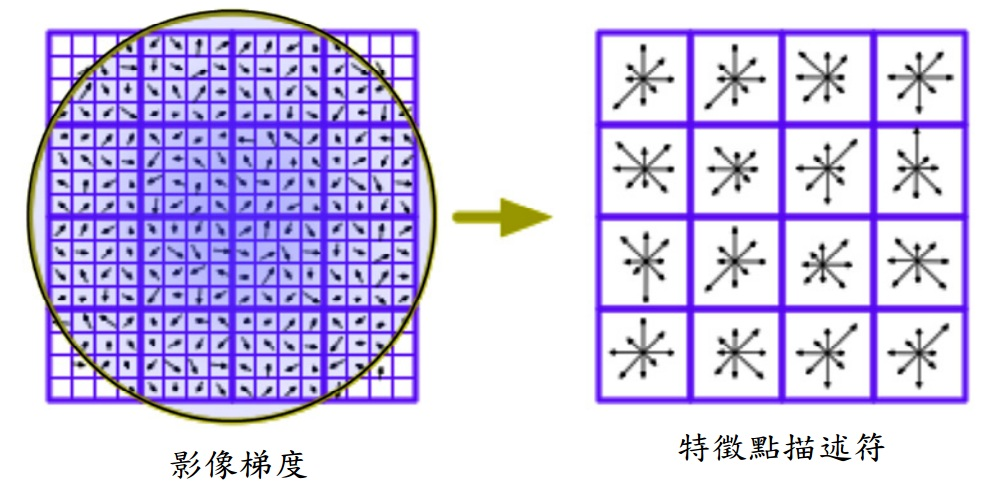
\includegraphics[width=0.8\textwidth]{figures/SIFT_histogram.jpg}
%  \caption{特徵點向量方為與強度示意直方圖}
%  \label{fig:SIFT Histogram}
%\end{center}
%\end{figure*}  
%
%     每個特徵點有 16 個方位的直方圖,每個方位直方圖內有 8 個梯度強度值,因此共有$16 x 8 = 128$個特徵值,
%     這些特徵點則為我們所需要的描述向量。

